%\documentclass[dvipdfmx,fleqn]{beamer}
\documentclass[dvipdfmx,fleqn,handout]{beamer}
\usepackage{amsmath,amssymb,amsthm}

\mode<presentation>
{
  \usetheme{Antibes}
  \usecolortheme{crane}
}

\title{\Large fictitious play}
\author{\large 小川紗里奈}
\date{\small }

\usefonttheme{professionalfonts}

\setbeamercovered{transparent=20}

\setbeamertemplate{navigation symbols}{} 
\setbeamertemplate{footline}[frame number] 



\begin{document}

\sffamily
\gtfamily


\begin{frame}
  \titlepage
  \thispagestyle{empty}
\end{frame}

\setcounter{framenumber}{0}




\begin{frame}\frametitle{はじめに}
 \begin{itemize}\setlength{\parskip}{0.5em}
  \item
  Fictitious playとは
  \item
  プログラムコード
  \item
  まとめ(今後の課題)
 \end{itemize}
\end{frame}



\begin{frame}\frametitle{Fictitious playとは}
 \begin{itemize}\setlength{\parskip}{0.5em}
  \item
  戦略形ゲームが $t=1,2,...$ の各期にプレイされるとする
  \item
  $t$期において各プレイヤーは、
  他のプレイヤーが$1$期から$t-1$期に選択した比率と等しい確率で各純粋戦略を選択すると予測
  →最適反応戦略を選択
  \item
  このような動学モデルをFictitious playという
 \end{itemize}
\end{frame}


\begin{frame}\frametitle{Fictitious playとは}
 \begin{itemize}\setlength{\parskip}{0.5em}
  \item
  各プレイヤーを0、1、戦略を0、1とする
  \item
  $t$期におけるプレイヤー0
   \begin{itemize}\setlength{\parskip}{0.5em}
    \item
    プレイヤー1は確率 $1-x_{0}(t)$ で0をとる
    \item
    プレイヤー1は確率 $x_{0}(t)$ で1をとる
    \item
    →この信念のもとで期待利得が最大になるような行動をとる
   \end{itemize}
  \item
  プレイヤー1も同様
 \end{itemize}
\end{frame}


\begin{frame}\frametitle{Fictitious playとは}
 \begin{itemize}\setlength{\parskip}{0.5em}
  \item
  初期信念 $x_{0}(0)$ は $[0,1]$ 上の一様分布に従いランダムに決まる
  \item
  各 $t \geq 1$ 時点においてプレイヤー1が過去にとった行動を $a_{1}(0),...,a_{1}(t-1)$ とすると
  \[
  x_{0}(t)
  = \frac{x_{0}(0) + a_{1}(0) + a_{1}(1) + ... + a_{1}(t-1)}{t + 1}
  \]

  ここで$x_{0}(t)$ は
  \[
  x_0(t+1)
  = x_0(t) + \frac{1}{t+2} (a_1(t) - x_0(t))
  \]
  と再帰的に書くことができる.
  これをプレイヤー0,1について考える
 \end{itemize}
\end{frame}


\begin{frame}\frametitle{Fictitious playとは}
 \begin{itemize}\setlength{\parskip}{0.5em}
  \item
  ただし
   \begin{itemize}\setlength{\parskip}{0.5em}
    \item
    $x_{0}(0),x_{1}(0) \sim Uniform[0,1]$
    \item
    $a_{0}(t)$ は $x_{0}(t)$ に対する最適反応、$a_{1}(t)$ は $x_{1}(t)$ に対する最適反応
    \item
    最適反応が複数ある場合は等確率でランダムに選ぶ
   \end{itemize}
 \end{itemize}
\end{frame}


\begin{frame}\frametitle{Fictitious playとは}
 \begin{itemize}\setlength{\parskip}{0.5em}
  \item
  例として次のようなMatching penniesゲームを考える
  \[
    \left[
     \begin{array}{rrr}
       1,-1 & -1,1 \\
       -1,1 & 1,-1
     \end{array}
    \right]
  \]
 \end{itemize}
\end{frame}


\begin{frame}[allowframebreaks,containsverbatim]\frametitle{プログラムコード}
 \begin{itemize}\setlength{\parskip}{0.5em}
  \item
  信念形成のシミュレーション
   \begin{verbatim}
   import matplotlib.pyplot as plt
   import random
   
   t = 1000
   x0 = random.uniform(0,1)
   x1 = random.uniform(0,1)
   
   x0_values = [x0]
   x1_values = [x1]
   profit = [(1,-1),(-1,1),(-1,1),(1,-1)]
    # [左上、右上、左下、右下]
   
   for i in range(t):
   
       if profit[0][0]*(1-x0) + profit[1][0]*x0
        > profit[2][0]*(1-x0) + profit[3][0]*x0:
            a0 = 0
       elif profit[0][0]*(1-x0) + profit[1][0]*x0
        < profit[2][0]*(1-x0) + profit[3][0]*x0:
            a0 = 1
       else:
            a0 = random.choice([0,1])
   
       if profit[0][1]*(1-x1) + profit[2][1]*x1
        > profit[1][1]*(1-x1) + profit[3][1]*x1:
            a1 = 0
       elif profit[0][1]*(1-x1) + profit[2][1]*x1
        < profit[1][1]*(1-x1) + profit[3][1]*x1:
            a1 = 1
       else:
            a1 = random.choice([0,1])
   
       x0 = x0 + (a1 - x0)/(i + 2)
       x1 = x1 + (a0 - x1)/(i + 2)
   
       x0_values.append(x0)
       x1_values.append(x1)
   
   plt.plot(x0_values, 'b-', label = 'x_0(t)')
   plt.plot(x1_values, 'r-', label = 'x_1(t)')
   plt.legend()
   plt.show()
   \end{verbatim}
  \item
  既存の信念をリストに加える
  →それをもとに期待利得を計算して戦略決定
  →その期の相手の行動から、さらに信念を更新
  を繰り返している
 \end{itemize}
\end{frame}


\begin{frame}\frametitle{信念のプロット}
 \begin{figure}
  \centering
  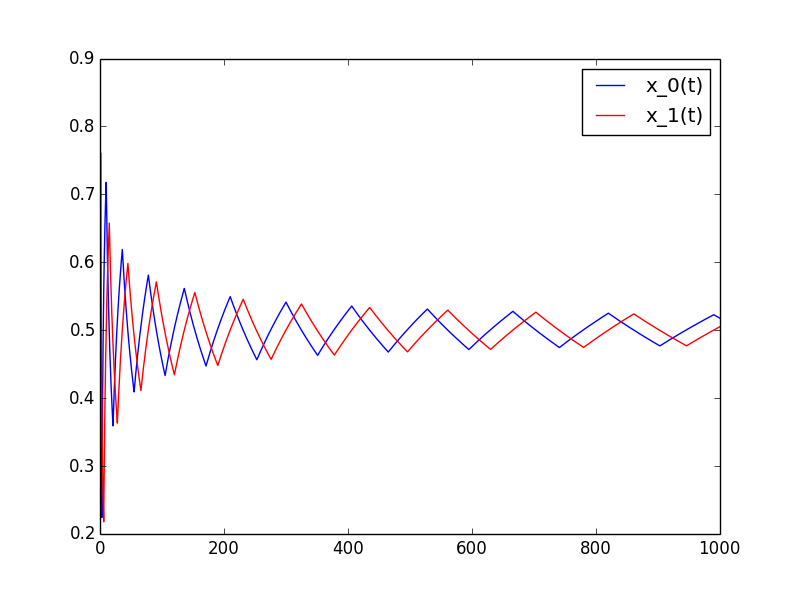
\includegraphics[width=7.5cm]{fictplay.pdf}
  \label{fig:fictplay}
 \end{figure}
  \begin{itemize}\setlength{\parskip}{0.5em}
   \item
   プレイヤーの信念は0.5付近に収束
  \end{itemize}
\end{frame}


\begin{frame}\frametitle{今後の課題}
 \begin{itemize}\setlength{\parskip}{0.5em}
  \item
  numpyを用いて利得を行列で計算するとよかった
  \item
  各プレイヤーの行動決定の際プレイヤー0と1で同じ過程を繰り返していたので
  関数としてまとめるべきだった
 \end{itemize}
\end{frame}



\end{document}